\documentclass{article}

\usepackage[a4paper, margin=1in]{geometry}
\usepackage[onehalfspacing]{setspace} % Correct 1.5 line spacing

\usepackage{graphicx}  % Figures
\graphicspath{{./figures/}}

\usepackage{url}
\usepackage[pdfusetitle]{hyperref}
\usepackage{titlesec}      % Modify title/section/chapter commands
\usepackage{mathtools}     % Various maths related commands
\usepackage{gensymb}       % \degree symbol
\usepackage[thinc]{esdiff} % Derivatives
\usepackage{booktabs}      % \toprule, etc., in tables
\usepackage{doi}           % support DOI links in bibliography
\usepackage{wrapfig}       % figures in text

\usepackage{fontspec}      % Fonts
\usepackage{helvet}
\usepackage{newpxtext,newpxmath}
\defaultfontfeatures{Scale=MatchLowercase, Ligatures=TeX}

\usepackage{algorithm}
\usepackage{algpseudocode}

% SI units
\usepackage{siunitx}
\sisetup{separate-uncertainty=true,number-mode=text,detect-weight=true}
\DeclareSIUnit\belm{Bm}
\DeclareSIUnit\belw{BW}
\DeclareSIUnit\beli{Bi}
\DeclareSIUnit\belz{BZ}

% https://tex.stackexchange.com/a/43009
\DeclarePairedDelimiter\abs{\lvert}{\rvert}%
\DeclarePairedDelimiter\norm{\lVert}{\rVert}%

% Caption figures
\usepackage{caption}
\DeclareCaptionFont{captionlabelfont}{\bfseries \sffamily}
\DeclareCaptionFont{captiontextfont}{\sffamily}
\captionsetup{labelfont=captionlabelfont, textfont=captiontextfont}

% Change footnote style
\renewcommand{\thefootnote}{\fnsymbol{footnote}}

% Fancy header/footer
\usepackage{fancyhdr}
\pagestyle{fancy}
\renewcommand{\sectionmark}[1]{\markright{\thesection . #1}}
\fancyhf{}
\lhead{\fancyplain{}{\thepage}}
\rhead{\fancyplain{}{\textit{\rightmark}}}

% Bibliography
\usepackage[backend=biber, style=ieee, natbib=true,
			url=false, isbn=true, doi=true,
			eprint=false, urldate=long]{biblatex}
%\addbibresource{references-old.bib}
\addbibresource{references.bib}

% biblatex IEEE style leaves empty parentheses when there is no date/year field.
% Since there are no date fields for many online resources, we use
%   https://tex.stackexchange.com/a/151264
% to stop these parentheses from being generated if there is no date field.
\usepackage{xpatch}
\xpatchbibdriver{online}
{\printtext[parens]{\usebibmacro{date}}}
{\iffieldundef{year}
	{}
	{\printtext[parens]{\usebibmacro{date}}}}
{}
{\typeout{There was an error patching biblatex-ieee (specifically, ieee.bbx's @online driver)}}

\renewcommand{\descriptionlabel}[1]{\hspace*{\labelsep}\spacedlowsmallcaps{#1}}

\titlespacing*{\chapter}{0pt}{1\baselineskip}{1.2\baselineskip}
\titlespacing*{\section}{0pt}{1.25\baselineskip}{1\baselineskip} 
\titlespacing*{\subsection}{0pt}{1.25\baselineskip}{1\baselineskip}
\titlespacing*{\paragraph}{0pt}{1\baselineskip}{1\baselineskip}

% Fix for missing µ in siunitx ???
% https://tex.stackexchange.com/a/428215
\sisetup{math-micro=\text{µ},text-micro=µ}

\newcommand\mytitle    {Millimetre-Wave Cloud Profiling Radar}
\newcommand\mysubtitle {Project Report}
\newcommand\myauthor   {180014855}
\newcommand\mydate     {\today}
\newcommand\mymodule   {PH4111}
\newcommand\mywordcount{2300}

\title {\mytitle}
\author{\myauthor}
\date  {\mydate}

%\usepackage[acronym,nonumberlist]{glossaries}
%\usepackage[acronym,nonumberlist]{glossaries-extra}

\usepackage[nopostdot, toc, nogroupskip, nomain, indexonlyfirst, acronym, symbols, style=long4col, stylemods={longextra}, nonumberlist, automake]{glossaries-extra}

\makeglossaries

%\setabbreviationstyle[acronym]{long-short}

\newacronym{ac:daq}{DAQ}{Data acquisition}
\newacronym{ac:simd}{SIMD}{Single instruction, multiple data}
\newacronym{ac:cpr}{CPR}{Cloud profiling radar}
\newacronym{ac:fmcw}{FMCW}{Frequency-modulated continuous wave}
\newacronym{ac:netcdf}{NetCDF}{Network common data form}
\newacronym{ac:openmp}{OpenMP}{Open multi-processing}
\newacronym{ac:adc}{ADC}{Analogue to digital converter}
\newacronym{ac:dds}{DDS}{Direct digital synthesiser}
\newacronym{ac:dft}{DFT}{Discrete Fourier transform}
\newacronym{ac:fftw}{FFTW}{Fastest Fourier Transform in the West}
\newacronym{ac:mkl}{Intel MKL}{Intel Math Kernel Library}
\newacronym{ac:snr}{SNR}{Signal-to-noise ratio}
\newacronym{ac:if}{IF}{Intermediate frequency}
\newacronym{ac:cpi}{CPI}{Coherent processing interval}
\newacronym{ac:cpu}{CPU}{Central processing unit}

%\newglossaryentry{busywaiting}
%{
%	name=formula,
%	description={A mathematical expression}
%}

\glsaddall

\begin{document}

\begin{titlepage}
	\centering
	{
\includegraphics[width=0.3\textwidth]{uos-logo}}
	\par
	{\LARGE\bfseries University of St Andrews\par}
	{\LARGE School of Physics and Astronomy\par}
	\vspace{1.5cm}
	{\huge\bfseries\mytitle\par}
	{\Large\mysubtitle\par}
	\vspace{2cm}
	{\Large\myauthor\par}
	{\large\textbf{Module:} \mymodule\par}
	{\large\textbf{Word count:} \mywordcount\par}
	\vfill
	{\large\today\par}
\end{titlepage}

\begin{abstract}
	Insert abstract here.
\end{abstract}

\tableofcontents

\section{Introduction}

\section{Signal processing theory}
\subsection{FMCW-Doppler radar}
Explain fast and slow time / range and velocity determination. Range and velocity resolution.

Is it worth including fig \ref{fig:Chirp}?
\begin{figure}
	\centering
	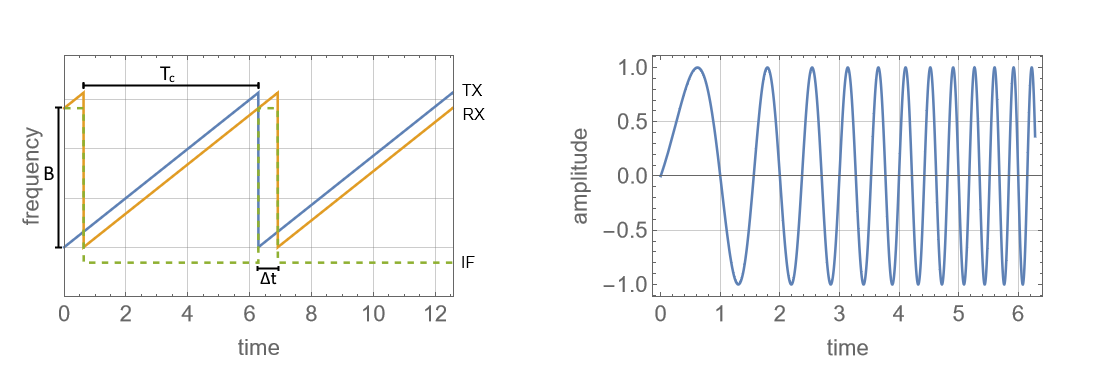
\includegraphics[width=\textwidth]{chirp}
	\caption{Chirp (own work)}
	\label{fig:Chirp}
\end{figure}

\begin{figure}
	\centering
	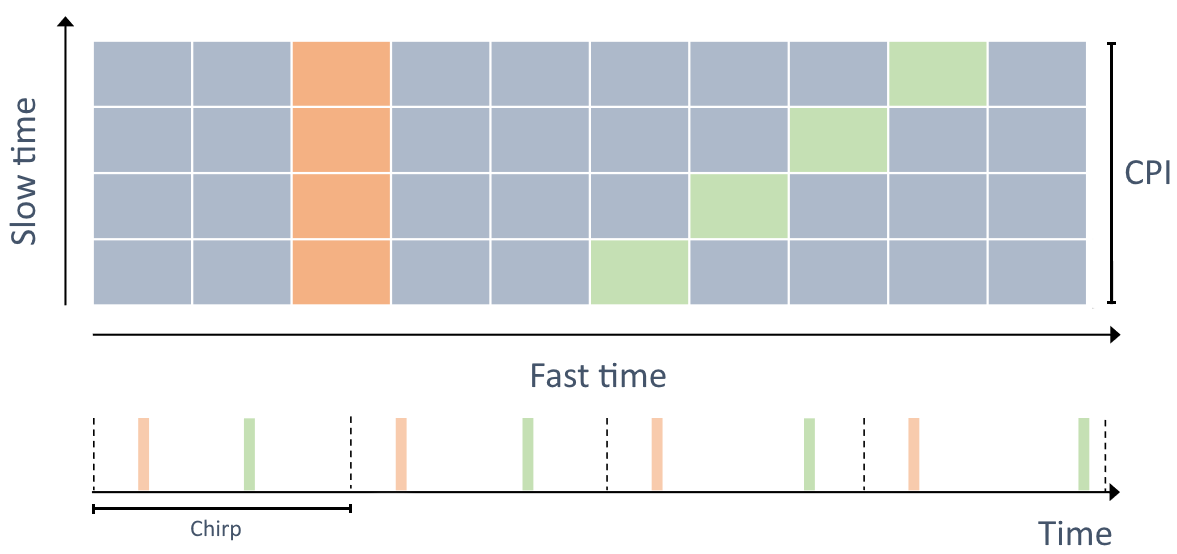
\includegraphics[width=\textwidth]{slow-fast-time}
	\caption{Fast-time vs slow-time. Adapted from \cite{SlowFastTimeFig}.}
	\label{fig:SlowFastTime}
\end{figure}

\subsection{Signal averaging}
Explain with signal averaging we can get \(\sqrt{N}\) improvement in SNR, why that's necessary to detect clouds

\begin{figure}
	\centering
	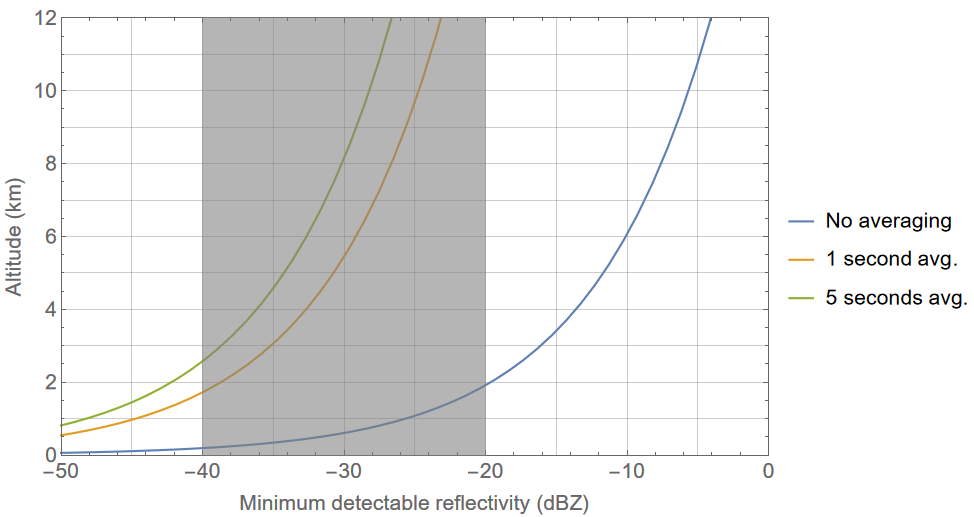
\includegraphics[width=0.6\textwidth]{sensitivity}
	\caption{Radar sensitivity  (Own work).}
	\label{fig:SlowFastTime}
\end{figure}

\subsection{Doppler moments}
I wonder if it's worth removing this section since I didn't quite get Doppler moments working

\section{Requirements}
Explain current state of Mark I and Mark II software


\begin{figure}
	\centering
	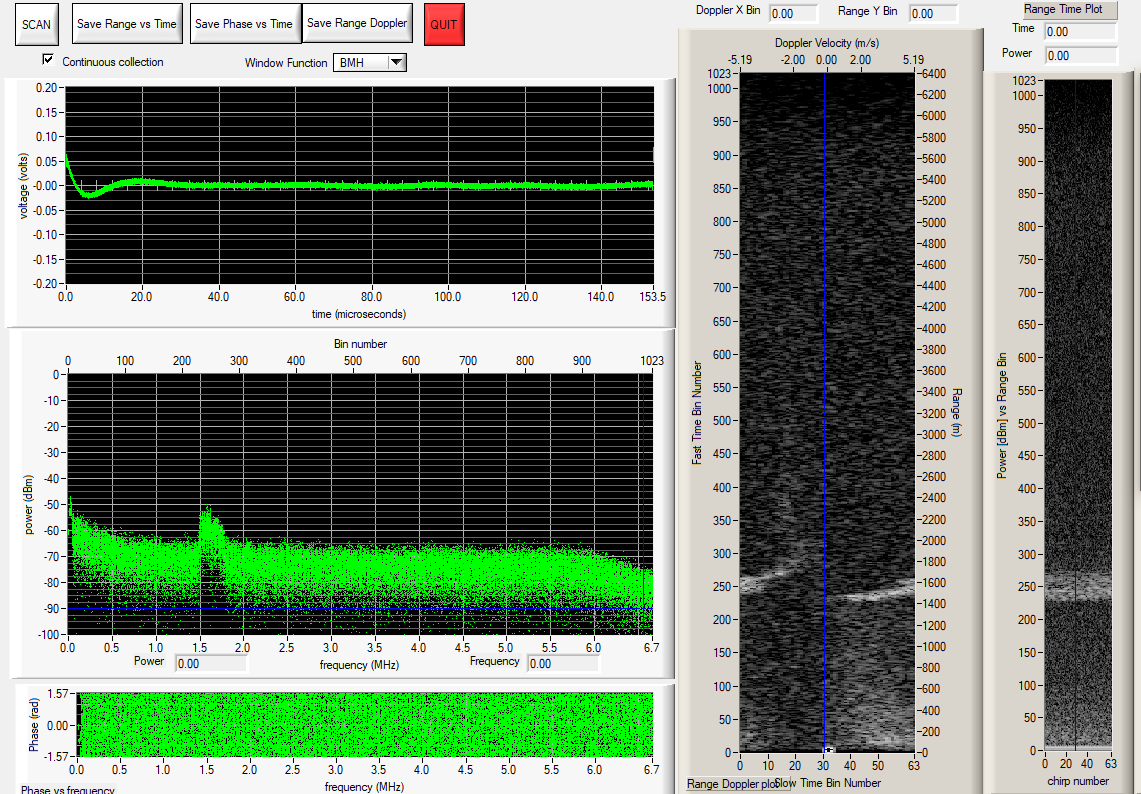
\includegraphics[width=\textwidth]{mark-1-rain}
	\caption{Screenshot of Mark I user interface, taken during precipitation.}
	\label{fig:Mark1Rain}
\end{figure}

\section{Design and implementation}
\begin{figure}
	\centering
	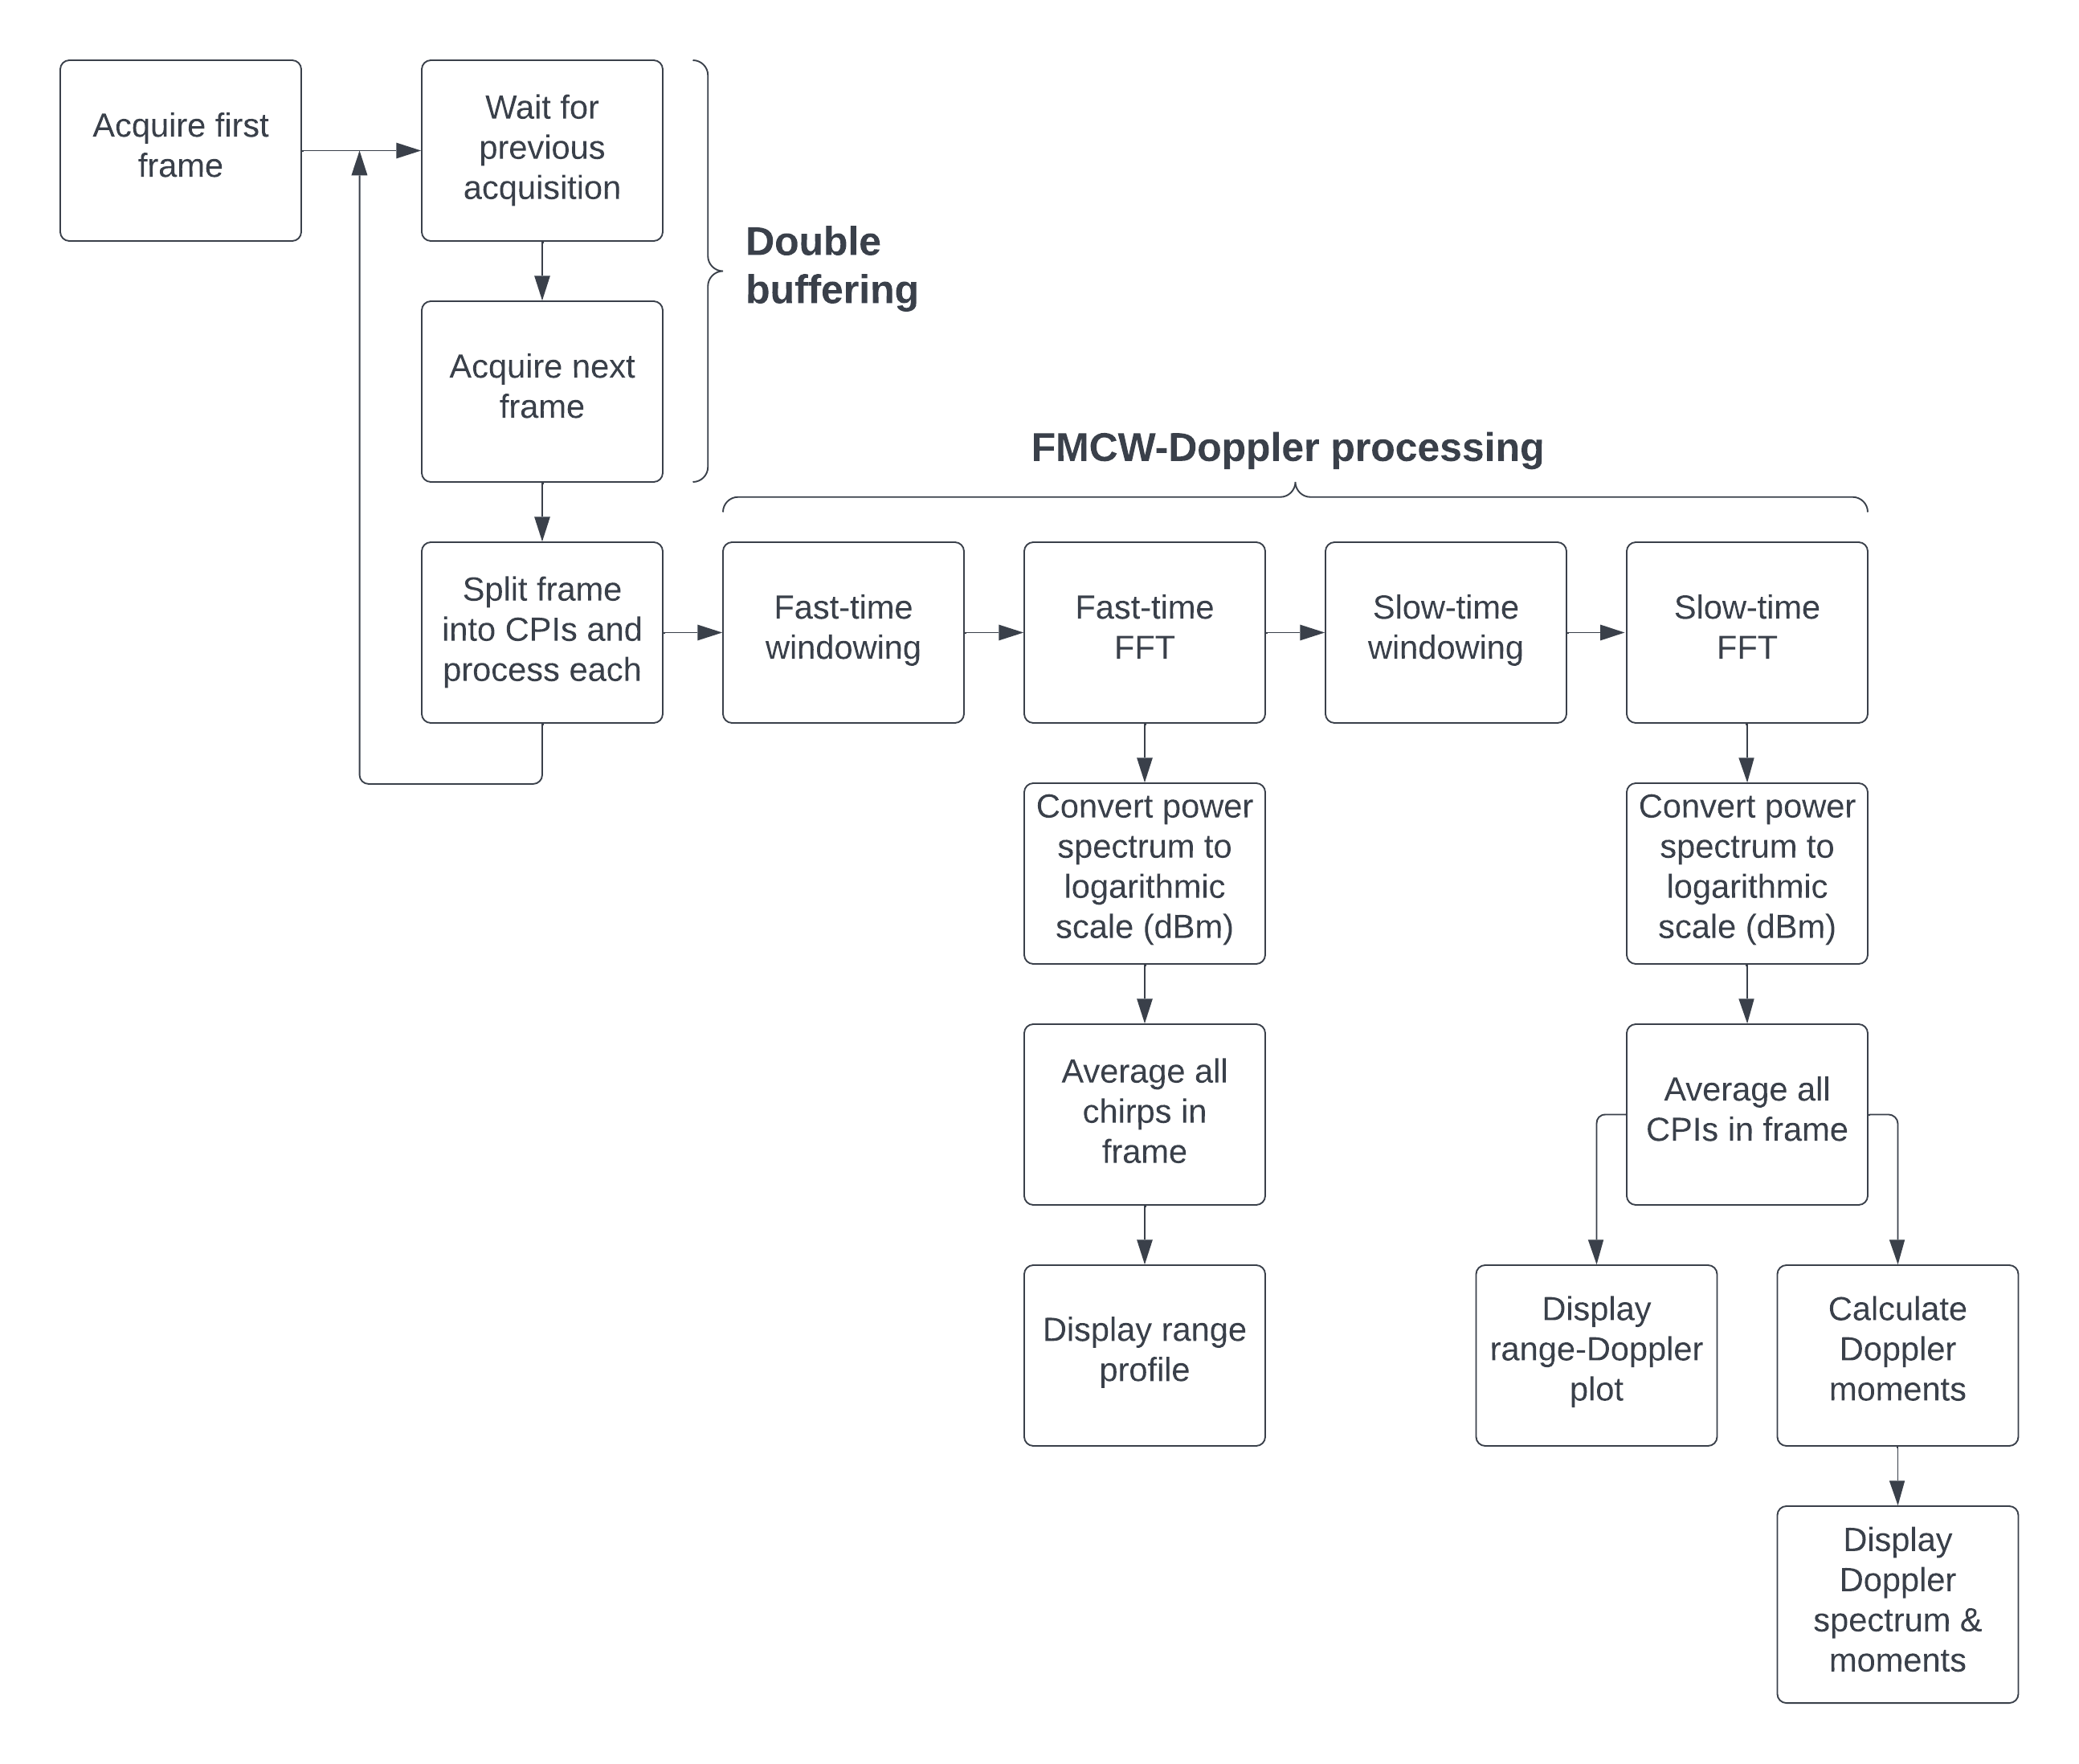
\includegraphics[width=\textwidth]{signal-processing-diagram}
	\caption{Simplified block diagram illustrating key signal processing steps. (Own work)}
	\label{fig:SignalProcessingDiagram}
\end{figure}

\subsection{Data acquisition}
\subsubsection{Double buffering}
To ensure real-time output, a double buffering approach is used.
One buffer is used to store the incoming frame and another stores the most recently acquired frame.
While the next frame is being acquired, the most recent frame is processed and displayed. The algorithm is shown in Alg. \ref{alg:DoubleBuffering}.

\begin{algorithm}
	\centering
	\begin{algorithmic}
		\State acquire frame asynchronously into buffer $A$
		\While {keep acquiring data}
		\State wait for previous acquisition to finish
		\State acquire frame asynchronously into buffer $B$
		\State process frame in buffer $A$
		\State display processed frame
		\State swap $A$ and $B$ pointers
		\EndWhile
	\end{algorithmic}
	\caption{Double buffering approach.}\label{alg:DoubleBuffering}
\end{algorithm}

\subsubsection{Alternatives to double buffering}
The approach in Mark II used one acquisition thread and one processing thread. The acquisition thread repeatedly acquires and appends frames to a thread-safe queue, which the processing thread pulls from.

The main issue with this approach is the acquisition thread wastes \acrshort{ac:cpu} time waiting for the frame to be acquired and transferred to memory.

\begin{algorithm}
	\begin{minipage}{0.48\linewidth}
		\begin{algorithmic}
			\While {keep acquiring data}
			\State acquire frame into buffer
			\State wait for previous acquisition to finish
			\State copy into thread safe queue
			\EndWhile
		\end{algorithmic}
	\end{minipage}
	\begin{minipage}{0.48\linewidth}
		\begin{algorithmic}
			\While {keep acquiring data}
			\State copy next frame in thread-safe queue
			\State process frame
			\State display processed frame
			\EndWhile
		\end{algorithmic}
	\end{minipage}
	\caption{Acquisition (left) and processing (right) threads.}\label{alg:TwoThreads}
\end{algorithm}

The double buffering approach uses only two buffers, which avoids unnecessary copying of data between threads and the additional overhead of using a thread-safe queue.

\subsection{FMCW-Doppler processing}
The software uses a third-party library, \acrshort{ac:fftw} v3\cite{FFTWv3}, to ensure correctness and good performance in the two discrete Fourier transform steps in the FMCW-Doppler process.

Newer versions of LabWindows CVI use \acrshort{ac:fftw} behind the scenes, however the interface is not as flexible. \acrshort{ac:fftw} supports multiple transforms of non-unit stride,\footnote{Stride is the number of memory locations between each successive element in an array.} allowing one to easily perform multiple transforms along different dimensions. This is particularly useful for the column-wise slow-time transform, because it means the data does not need to be transposed before transforming.


The window functions available in the new software are flat-top, Han, Blackman, and Blackman-Harris.

\subsubsection{Averaging}
In each frame, two averaging processes take place. Averaging of power spectra is done over each chirp. For a frame containing \(256\) \acrshort{ac:cpi}s each containing \(64\) chirps, this amounts to \(256 \times 64 = \)

\subsection{Testing}
To facilitate testing the software, a mock implementation of the \acrshort{ac:daq} was created. Raw data (\acrshort{ac:adc} integers) saved by the Mark II can be loaded by the mock implementation and used as if the data was just acquired. This feature is extremely useful for reproducible debugging and testing. A few snapshots of rain data were saved and used to test the new code when the weather was too clear.

A signal generator was attached to the second input channel of the \acrshort{ac:daq} card. Checking to see if the input power matches the peak value in the fast-time power spectrum provides confirmation that any corrections or scaling performed during the fast-time processing is correct.

Setting the input frequency to be slightly off bin centre introduces spectral leakage (Fig. \ref{fig:WindowNone}) Fig. \ref{fig:WindowBMH} shows the effect of applying the Blackman-Harris window is as expected.

\begin{figure}
	\centering
	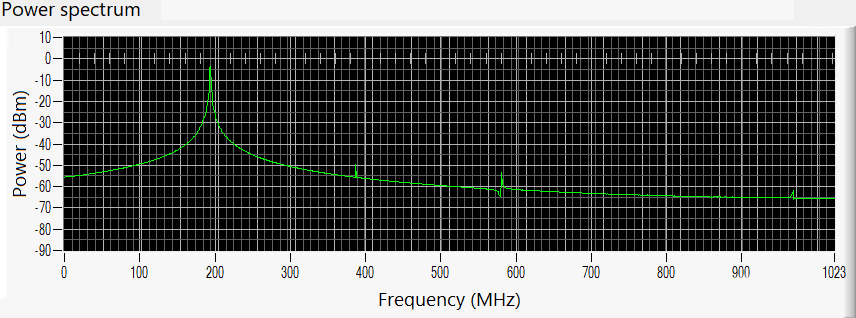
\includegraphics[width=\textwidth]{window-none}
	\caption{Fast-time power spectrum without windowing.}
	\label{fig:WindowNone}
\end{figure}

\begin{figure}
	\centering
	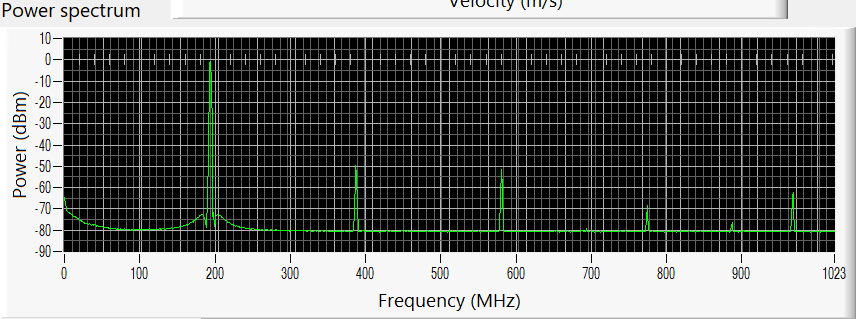
\includegraphics[width=\textwidth]{window-bmh}
	\caption{Fast-time power spectrum with Blackman-Harris windowing.}
	\label{fig:WindowBMH}
\end{figure}

\subsection{Averaging}
How is averaging implemented? Not much to say here really

\section{Results}

\begin{figure}
	\centering
	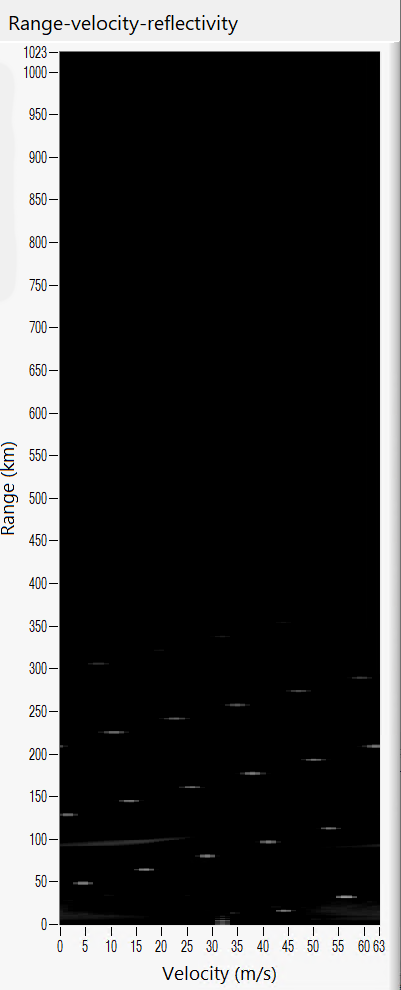
\includegraphics[width=0.4\textwidth]{working-cloud_range-doppler}
	\caption{Screenshot of the new user interface.}
	\label{fig:WorkingCloudRangeDoppler}
\end{figure}

\begin{figure}
	\centering
	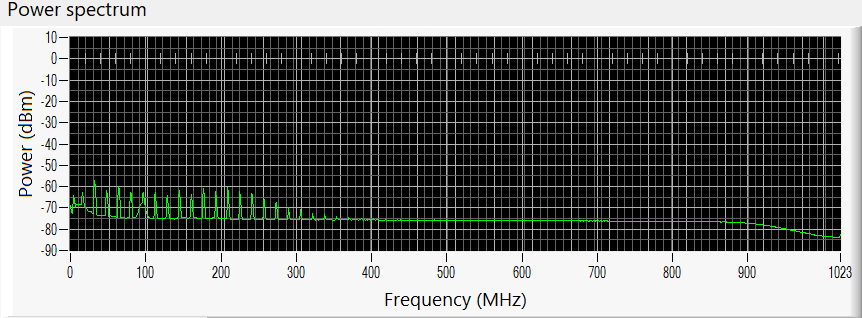
\includegraphics[width=\textwidth]{working-cloud_power-spect}
	\caption{Screenshot of the new user interface.}
	\label{fig:WorkingCloudPowerSpectrum}
\end{figure}

\begin{figure}
	\centering
	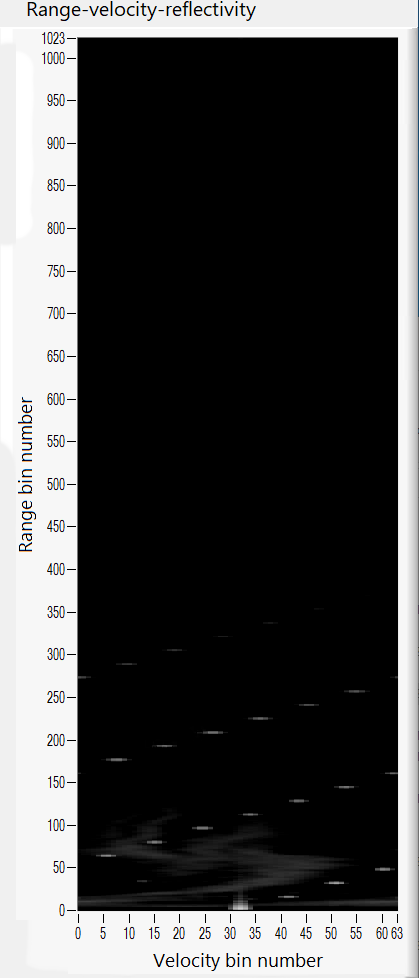
\includegraphics[width=0.4\textwidth]{working-hail_range-doppler}
	\caption{Screenshot of the new user interface.}
	\label{fig:WorkingHailRangeDoppler}
\end{figure}

\begin{figure}
	\centering
	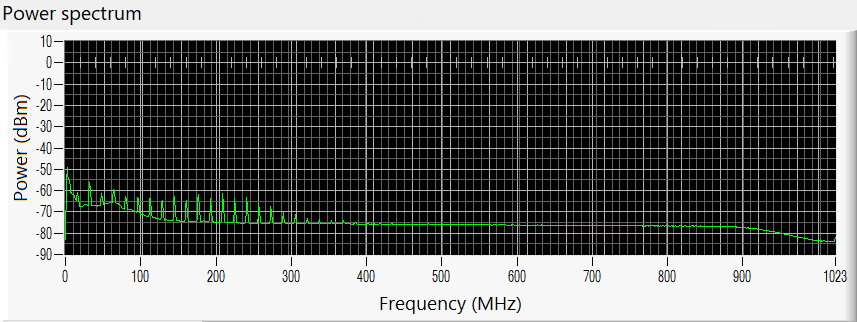
\includegraphics[width=\textwidth]{working-hail_power-spect}
	\caption{Screenshot of the new user interface.}
	\label{fig:WorkingHailPowerSpectrum}
\end{figure}

\begin{figure}
	\centering
	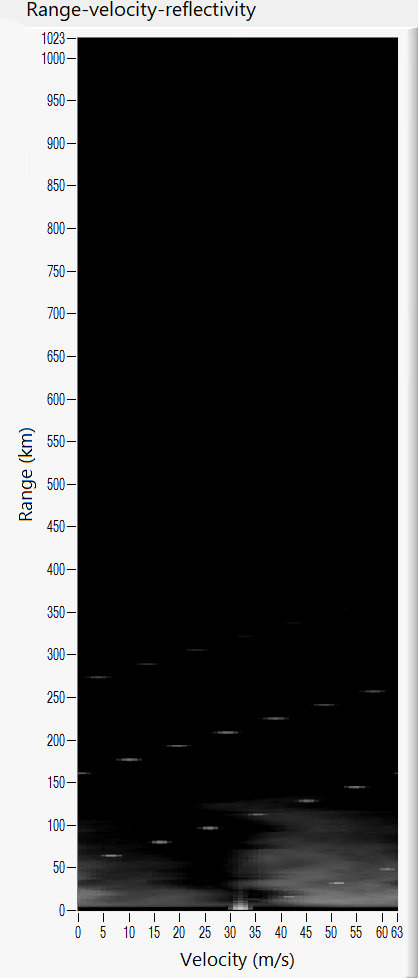
\includegraphics[width=0.4\textwidth]{working-heavy-rain-sleet_range-doppler}
	\caption{Screenshot of the new user interface.}
	\label{fig:WorkingHeavyRainSnowRangeDoppler}
\end{figure}

\begin{figure}
	\centering
	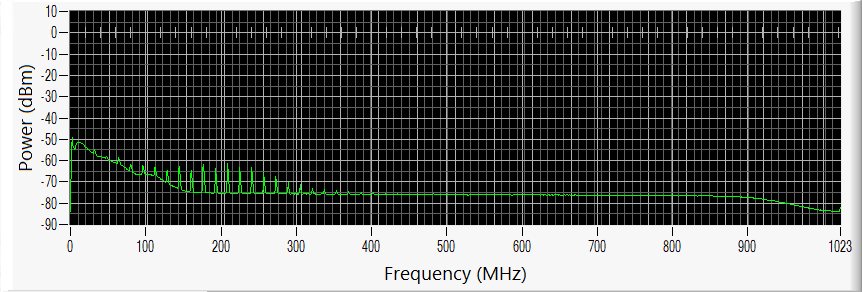
\includegraphics[width=\textwidth]{working-heavy-rain-sleet_power-spect}
	\caption{Screenshot of the new user interface.}
	\label{fig:WorkingHeavyRainSnowPowerSpectrum}
\end{figure}

\subsection{Performance}
Compare processing time of previous software

\section{Future work}
\subsection{Doppler moments}
Extracting the Doppler spectrum from the averaged range-Doppler data has already been implemented along with UI controls for displaying Doppler moments, however the formulas used for determining the moments are incorrect.

\subsection{Effect of ambient temperature}
\subsection{NetCDF}

\subsection{Performance improvements}
\subsubsection{Multithreading}
An easy way of using multithreading is \acrshort{ac:openmp}
[Briefly mention how OpenMP can be used to parallelise loops]

\subsubsection{SIMD}
Single instruction, multiple data (SIMD) is another type of parallel processing where a single instruction operates simultaneously on multiple pieces of data. \acrshort{ac:fftw} uses this extensively. Many of the steps in the FMCW-Doppler process are adding or multiplying rows or columns by the same constants which makes \acrshort{ac:simd} ...

\section{Conclusions}

\clearpage
\printglossary
\printbibliography

\end{document}
